%As a result of allowing inexact matches, there may be multiple fragments in an optical map that could each be a reasonable match for an {\em in silico} digested fragment, and in order to include all of these as candidate matches, backtracking becomes necessary in the backward search.
%For every backward search path that maintains a non-empty interval for the entire query contig, we emit the alignments denoted by the final interval.%, mapped back to a position in the optical map.

\begin{figure*}[h!]
 \centering
 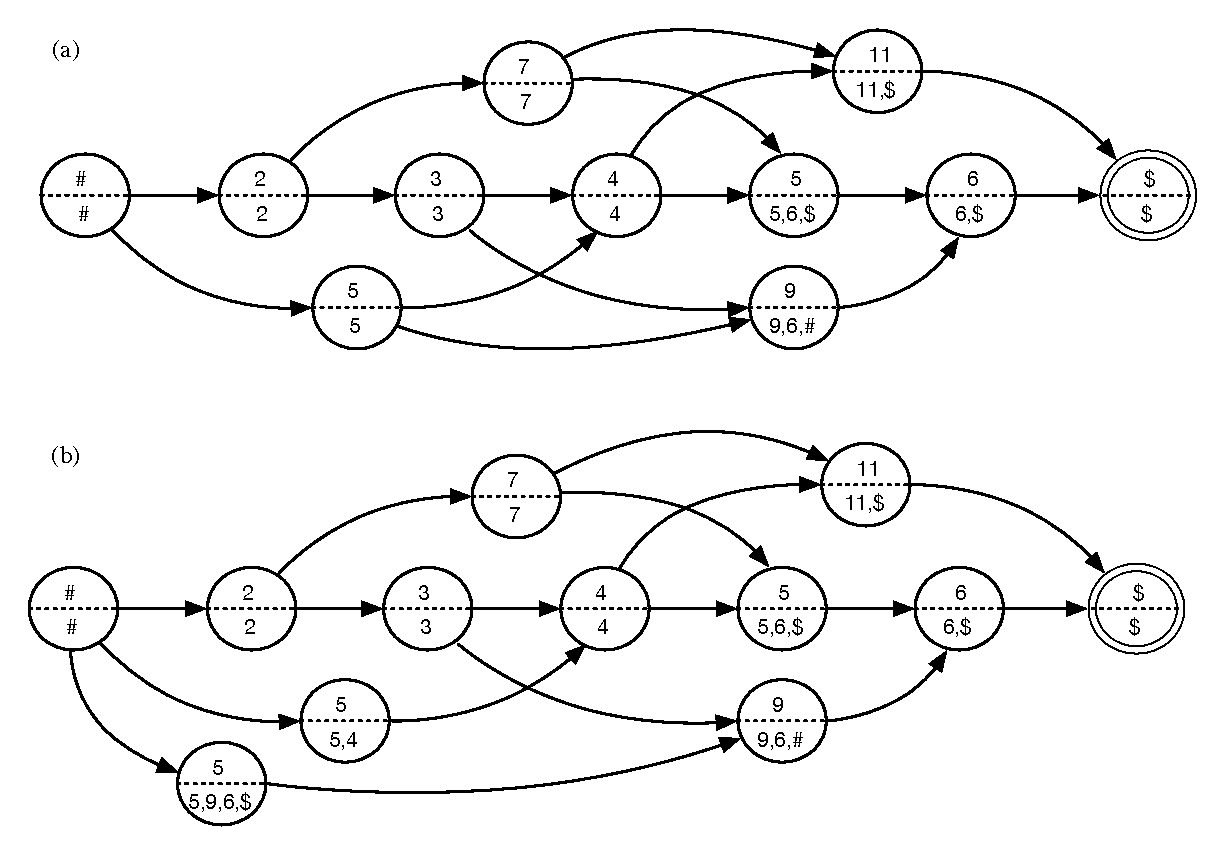
\includegraphics[width=0.6\textwidth]{../content/figures/example_combined}
  \caption{(a) shows an example automaton.  The top half of vertices contains the label, which models a fragment size in Kbp.  The common prefixes of all suffixes spelled from a vertex is written in the bottom half.  Note that there is no ordering of vertices such that all their corresponding suffixes are in lexicographic order;  the leftmost vertex labelled with ``5'' spells suffixes beginning ``5,4,...'' as well as the suffix ``5,9,6,\$'' while the rightmost $5$  spells the suffix ``5,6,\$''. (b) shows the prefix sorted automaton corresponding to the one in (a).  The leftmost vertex $5$ has been duplicated and the outgoing edges of the previous version have been divided between the new replacement instances.  This also divides the suffixes spellable from the prior version.  Now the three $5$ vertices can be ordered based on their common prefixes as [``$5$,$4$,...'',``$5$,$6$,\$'', ``$5$,$9$,$6$, \$'']. }
\label{fig:example}
\end{figure*}

\begin{table*}[h!]
\begin{center}
  \begin{tabular}{ccccccccccccc}
  	\hline
		& \$		& 2		& 3		& 4		& 5,4		& 5,6,\$	& 5,9,6,\$	& 6,\$	& 7	& 9,6,\$	& 11,\$	& \# \\
	\hline
$\BWT$	& 6,11	& \#		& 2		& 3,5		& \#		& 4,7		& \#		& 5,9		& 2	& 3,5		& 4,7		& \$ \\
$\M$		& 1		& 10		& 10		& 10		& 1		& 1		& 1		& 1		&10	& 1		& 1 		& 100 \\
$\F$		& 10		& 1		& 1		& 10		& 1		& 10		& 1		& 10		& 1	& 10		& 10		& 1 \\		
	\hline
	\end{tabular}
      \caption{Table listing the three arrays storing the automaton in memory: $\BWT$, $\M$, and $\F$.}
 \label{bwt-table}
\end{center}
\end{table*}


\subsection{Generalized Compressed Suffix Array.}

%It is an extension of the {\em XBW transform}~\cite{xbw}, which is a compressed  index structure for labeled trees that in itself is a generalization of the FM-index~\cite{dag_method}.  It is an extension of the {\em XBW transform}~\cite{xbw}, which is a compressed  index structure for labeled trees that in itself is a generalization of the FM-index~\cite{dag_method}.  

We index the automaton with the GCSA~\cite{dag_method} for efficient storage and path querying.  The GCSA is a generalization of the FM-index for automata and
%---which as previously mentioned, only supports indexing and querying strings. Nonetheless, there are some parallels between the two data structures and 
we will explain the GCSA by drawing on the definition of the (more widely known) FM-index.  As stated in the background section, the FM-index is based on the deep relationship between the $\SA$ and the $\BWT$ data structures of the input string $\X$. The $\BWT$ of an input string is formed by sorting all characters of the string by the lexicographic order of the suffix immediately following each character.  The main properties the FM-index exploits in order to perform queries efficiently are a) $\BWT[i] = \X[\SA[i]-1]$; and 
%b) the index in the $\SA$ that starts with a given symbol can be found from the $\BWT$ index containing that symbol using small auxiliary data structures. 
b) given that $\SA[i] = j$, and $\C[c]$ gives the position of the first suffix in $\SA$ prefixed with character $c$, then using small auxiliary data structures we can quickly determine $k = \C[\BWT[i]] + \rank(\BWT,\BWT[i],i)$, such that $\SA[k] = j-1$.
The first of these properties is simply the definition of the $\BWT$.  The second is, because the symbols of $\X$ occur in the same order in both the single character prefixes in the suffix array and in the $\BWT$, given a set of sorted suffixes, prepending the same character onto each suffix does not change their order. Thus, if we consider all the suffixes in a range of $\SA$ which are preceded by the same symbol $c$, that subset will appear in the same relative order in (another part of) $\SA$: as a contiguous subinterval of the interval that contains all the suffixes beginning with $c$. Thus by knowing where a symbol's run begins in the $\SA$ and the $\rank$ of an instance of that symbol, we can identify the $\SA$ position beginning with that instance from its position in $\BWT$. A rank data structure over the $\BWT$ thus constitutes a compressed version of the suffix array. 
%The FM-index $\LF()$ function computes the $\SA$ position from the $\BWT$ position using these auxiliary data structures.

%Because those suffixes with the same single character left extension would occur in the same order as those suffixes without the extension, there is a relationship between each suffix and the next longer suffix.  
%Because the BWT is created from sorted suffixes, each position in the BWT can be treated as denoting a particular suffix in a suffix array.  The preceeding character of each suffix is also the one found in the BWT itself for the position in the BWT that denotes that suffix.


%The possition in the equivalent suffix array that represents the $c$ extension can be found using two auxiliary data structures: 1) a $C$ array storing the count of all the lexicographically smaller characters in the text, which can be used to find the beginning of that run of suffixes beginning with that character in the suffix array and 2) an $Occ$ array storing for each position in in the BWT, how many instances of a given character preceed that position.  Since these symbols in the BWT are the prefix characters of the suffixes in the suffix array, they will be in the same order as their sorted -1 suffixes, so their relative position gives an offset into the run of that character prefixes in the suffix array.  $Occ$ is equivalent to the \rank of those characters.  These combination of the start of the run in the SA (given by $C$) and the offset into that run (given by $Occ$) allows mapping from positions in BWT that match a suffix to posstions that denote a $c$ extension.  

%If we allow a suffix array to encode rotations instead of suffixes of a text, the sorted set of rotations can form the Burrows-Wheeler Matrix with the last column being the BWT.  The operation for computing the position of a $c$ extension is called LF() for last-to-first, as it takes the position of a character in the last column of this matrix and computes its position in the first column. 

To generalize the FM-index to automata (from strings), we need to efficiently store the vertices and edges in a manner such that the FM-index properties still hold, allowing the GCSA to support queries efficiently.  An FM-index's compressed suffix array for a string $S$ encodes a relationship between each suffix $S$ and its left extension.  Hence, this suffix array can be generalized to edges in a graph that represent a relationship between vertices.  The compressed suffix array for a string is a special case where the vertices are labeled with the string's symbols in a non-branching path. %Now, we will describe this generalization in more detail by describing how to sort all vertices and edges in an automaton using $\BWT$ and two bit arrays.

\paragraph{Prefix-sorted automata.}
Just as backward search for strings is linked to suffix sorting, backward searching in the BWT of the automaton 
requires us to be able to sort the vertices (and a special set of the paths) of the automaton in a particular 
way. In~\cite{dag_method} this property is called {\em prefix-sortedness}. Let $A = (V,E)$ be a finite automaton, 
let $v_{|V|}$ denote its terminal vertex, and let $v \in V$ be a vertex. We say $v$ is {\em prefix-sorted} by 
prefix $p(v)$ if the labels of all paths from $v$ to $v_{|V|}$ share a common prefix $p(v)$, and no path from any 
other vertex $u \ne v$ to $v_{|V|}$ has $p(v)$ as a prefix of its label. Automaton $A$ is prefix-sorted if all 
vertices are prefix-sorted. See Figure~\ref{fig:example} for an example of a non-prefix sorted automaton and a 
prefix sorted automaton. A non-prefix sorted automaton can be made prefix sorted through a process of duplicating 
vertices and their incoming edges but dividing their outgoing edges between the new instances (see~\cite{dag_method}).

Clearly the prefixes $p(v)$ allow us to sort the vertices of a prefix-sorted automaton into lexicographical 
order. Moreover, if we consider the list of outgoing edges $(u,v)$, sorted by pairs $(p(u),p(v))$, they are
also sorted by the sequences $\ell(u)p(v)$, where $\ell(u)$ denotes the label of vertex $u$. This (dual sortedness)
property allows backward searching to work over the list of vertex labels (sorted by $p(v)$) in the same way
that is does for the symbols of a string ordered by their following suffixes in normal backward search for 
strings.

Each vertex has a set of one or more preceding vertices and therefore, a set of predecessor labels in the 
automaton. These predecessor label sets are concatenated to form the $\BWT$. The sets are concatenated the 
order defined by the above mentioned lexicographic ordering of the vertices. Each element in $\BWT$ then 
denotes an edge in the automaton. Another array of bits, $\F$, marks a `1' for the first element of $\BWT$ 
corresponding to a vertex and a `0' for all subsequent elements in that set. Thus, the predecessor labels, 
and hence the associated edges, for a vertex with rank $r$ are $\BWT[\select(r)..\select(r+1)]$. Another 
array, $\M$, stores the out degree of each vertex and allows the set of vertex ranks associated with a $\BWT$ 
interval to be found using $\rank()$ queries.

%\textit{Vertex Representation}
%In order to index the vertices we first construct an unique string, which we refer to as the \emph{common prefix}, and associate each vertex with respect to that string. This association will allow the vertices to be sorted by their common prefixes and from then on identified by their rank in this sorted order.  To construct the common prefix string, it is important to note that the automaton defines a language comprising a set of strings.  Thus, every path through the automaton corresponds to one of these strings.  If we consider all of the paths that include a particular vertex, we see that the vertex will also be the initial symbol of a suffix for each path.  Those suffixes will have a common prefix--even if it is just the node label itself--which is the common prefix string. 
%
%These common prefixes may not be sufficient to sort vertices as necessary.  In some cases, two vertices may share a property that all paths reachable from one are lexicographically smaller than all paths reachable from the other.  A vertex that shares this property with every other vertex is prefix sorted.  An automaton where every vertex is prefix sorted is a prefix sorted automaton.  A non-prefix sorted automaton can be made prefix sorted through a process of duplicating vertices and their incoming edges but dividing their outgoing edges between the new instances.  See Figure~\ref{fig:example} for an example of a non-prefix sorted automaton and a prefix sorted automaton.  The common prefix of these vertices will then be longer, and with sufficient repetitions of this process, a non-prefix sorted automaton will become prefix sorted. Thus, in order to ensure the vertices can be identified by their rank in sorted order, we construct the automaton so that it is prefix sorted. 
%
%\textit{Edge Representation}
%Each vertex has a set of one or more preceding vertices and therefore, a set of predecessor labels in the automaton.  These predecessor label sets are concatenated to form the $\BWT$ array.  
%The sets are concatenated in an order defined by the above mentioned lexicographic ordering of the vertices.
%%The order of concatenation among these sets is based on the aforementioned lexicographic rank of the successor of each set. 
%Each element of $\BWT$ then denotes an edge in the automaton.  Another array of bits, $\F$, marks a `1' for the first element of $\BWT$ corresponding to a vertex and a `0' for all subsequent elements.  Thus, the predecessor labels, and hence the associated edges, for a vertex with rank $r$ are $\BWT[\select(r)..\select(r+1)]$. Another array, $\M$, stores the out degree of each vertex and allows the set of vertex ranks associated with a $\BWT$ interval to be found using $\rank()$ queries.
%%A bit vector, $F$, is used to encode the mapping from vertex space to edge space, and a bit vector, $M$, is used to map from edge space back to vertex space.  Equivalently, these encode the in-degree and out-degree of the vertices.
%%Since there can be multiple characters preceeding a vertex (and thus all reachable paths from that vertex), a bit vector $F$ encodes with a '1' the first symbol in the BWT array which preceedes a common prefix vertex.  It allows us to map from  multiple BWT positions to a single SA position.  Just as with compressed suffix arrays, the actual suffix array is not stored in memory.% FIXME: describe M bit vector operation
%

% An automaton may be such that the possible suffixes reachable from two or more vertices, when sorted, have overlapping ranges (e.g. A path prefix vertex ``12'' may be followed by either a ``5'' or a ``9'' in one part of the automaton while ``12'' may be followed by either a ``4'' or a ``7'' elsewhere.  These vertices cannot be sorted according to the lexicographic order of reachable paths.)   To induce the required property of a definite ordering, we can modify the automaton by replacing vertices with short common prefixes using new vertices with longer, more specific, common prefixes (e.g. replace the original ``12'' prefix vertex with a ``125'' and a ``129'' vertex, and the latter with ``124'' and ``127'', thus these four vertices can be ordered.).  As vertices denoting short path prefixes are replaced with several longer path prefix vertices, eventually a definite ordering is induced.    This is called {\em prefix doubling}.

%Siren et al.~\cite{dag_method} show that the GCSA can be constructed in $O(|V|+|E|)$ time and space, where $|V|$ is the number of vertices in the automaton and $|E|$ is the number of edges. %Hence, it follows from this result that the automaton for the Rmap data can be constructed in $O(XX)$-time and $O(XX)$-memory.   
 %FIXME: this needs more work

%I don't think you need this --> In this discussion, we assume that the automaton was ensured to be reverse deterministic such that any member of $\Sigma$ only exists once labeling a predecessor vertex of each vertex.

% FIXME: look up proper orthographic form for burrows wheeler



%An FM-index allows exact string search because it encodes the relationship between each pair of consecutive symbols in a text.  The generalization of the GCSA is that the encoded relationship is between vertices in a directed graph.  Under this generalization, an FM-Index is just the special case of a graph formed where every symbol has a single in edge that originates at its predecessor in the text and a single out edge destined for its successor in the text.  The GCSA still includes the BWT component, and like FM-index backward search, an interval on a BWT can denote a subset of the indexed data.  

%In the FM-index, this interval has an equivalent interpretation in a suffix array and in this interpretation, a prefix of all strings in the interval match the suffix of the query searched up to that point.  In the GCSA, each element in the BWT corresponds to vertex in an automaton.  Each vertex has an annotated string indicated the longest common prefix of all strings reachable from it moving forward.  The interval then encodes all vertices whose prefix is consistent with the portion of the query matched up to that point.  

%After the construction of the GCSA, a wavelet tree $\M$ is created that allows us to map from positions in $\R_q$ to positions in $\R^*$ in constant time.

 
%Additional vertices are added to represent hypothetical fragments that could exist for every boundary between two (or more) fragments formed by successful enzyme digestion.  The hypothetical vertices of two combined fragments provide  alternative path segments (consisting of single vertices) around pairs of vertices in the backbone.


\subsection{Exact Matching: GCSA Backward Search.}

%Recall that our aim to find all $\R_i$ in the target database whose alignment to $\R_q$ has a Chi-square statistic less than $\rho_U$, and a ratio of matched to missed restriction sites greater than $\rho_L$.  

Exact matching with the GCSA is similar to the standard FM-index backward search algorithm. As outlined in the background section, FM-index backward search proceeds by finding a succession of lexicographic ranges that progressively match longer and longer suffixes of the query string, starting from the rightmost symbol of the query. The search maintains two items --- a lexicographic range and an index into the query string --- and the property that the path prefix associated with the lexicographic range is equal to the suffix of the query marked by the query index. Initially, the query index is at the rightmost symbol and the range is $[1..n]$ since every path prefix matches the empty suffix.  The search continues using GCSA's backward search step function, which takes as parameters the next symbol (to the left) in the query (i.e. fragment size in $\R_q$) and the current range, and returns a new range.  The query index is advanced leftward after each backward search step.  In theory, since the current range corresponds to a consecutive range in the $\BWT$, the backward search could use use $\select()$ queries on a bit vector $\F$ to determine all the edges adjacent to a given vertex and then two FM-index $\LF()$ queries are applied to the limits of the current range to obtain the new one.  GCSA's implementation uses one succinct bit vector per alphabet symbol to encode which symbols precede a given vertex instead of $\F$.  Finally, this new range, which corresponds to a set of edges, is mapped back to a set of vertices using $\rank()$ on the $\M$ bit vector.


%Each additional symbol in the query string is matched in a process taking two arguments: 1) a lexicographic range, the $\Y$-interval, corresponding to the suffixes in the text, $\ell$, whose prefix matches a suffix of the query string, and 2) an extension symbol $c$.  The process returns a new interval, the $c\Y$-interval, where the prefix of each text suffix corresponding to the new interval is a left extension of the previous query suffix. This works because each prefix of an alignment is also an alignment, including the base case of an empty prefix.





\subsection{Inexact Matching: GCSA Backward Search Using a Wavelet Tree.}


%We emphasize that for ease of exposition, the description of our modifications to and use of the GCSA in the remainder of this section  avoid specific differences between GCSA-based backward search and FM-index backward search. We thus talk about backward searching in the  GCSA as operations on the $\BWT$ of $\R^*$, etc.. We refer the reader interested in the fine-grained differences between the GCSA and FM-index to~\cite{dag_method}. 
% Muggli et al.~\cite{wabi2014} showed that a wavelet tree can efficiently find suitably sized substitute fragments over a large alphabet, but its basic FM-index structure cannot encode alternative compound fragments as substition candidates in light of missing site errors.

% C: this paragraph is too long, make shorter or split in two
%As previously mentioned,  GCSA was developed for sequences on a nucleotide alphabet.  

We modified backward search in the following ways:
(1) we used a wavelet tree to allow efficient retrieval of substitution candidates; (2) we modified the search process to combine consecutive query fragments into compound fragments so as to match fragments in $\R^*$ missing the interposing restriction site; and (3) we introduced backtracking, in order to try substitution candidates and combinations of compound fragment. These modifications are further detailed below.

First, in order to accommodate possible errors in fragment size, we determine a set, $\D$, of candidate fragment sizes that are similar to the next fragment of $\R_q$ to be matched in the query. These candidates are determined by enumerating the distinct symbols in the currently active backward-search range of the $\BWT$ using the wavelet tree algorithm of Gagie et al.~\cite{GNPtcs11}.  This requires introducing bit array $\F$ into the actual implementation\footnote{Recall that this active range, when applied to a lexicographic range, represents the suffixes whose prefixes are the matched portion of the query, while the same range of the $\BWT$ contains possible extension symbols.}. To accommodate possible restriction sites that are present in the query Rmap but absent in target Rmaps, we generate compound fragments (i.e. new symbols) by summing pairs and triples of consecutive query fragment size and then querying the wavelet tree for substitutions of these compound fragments. This summing of multiple consecutive fragments is complementary to the skip vertices in the target automaton and accommodates missed restriction sites in the target, just as the skip vertices accommodate missed sites in the query.  %We remove small fragments with a larger threshold than used for skip edge introduction.  This ensures no need for complementary handling of inconsistent desorption.


%We introduce skip {\emph edges} to provide paths around small target fragments which may be missing in the query.  We filter out small query fragments using a larger threshold to bias toward this scenario. 

%Similarly, small fragments may sometimes be subject to desorption in either the query or the target.
%SJP: found this next part a little wordy:
%One could simply prune all the fragments below a certain threshold size; however, due to the sizing error, one cannot discard based on the true fragment size and one would certainly not achieve consistent discarding across all Rmaps (e.g. a small fragment in two maps covering the same genomic region may be above the threshold in one map and below in another, leading to inconsistent discarding).  Therefore, to find all alignments, 
%and so
%some mechanism to allow inconsistent inclusion of small fragments is required.
%In order to allow inconsistent inclusion between query and target, we introduce skip edges.  These allow paths around small fragments found in the target that might be missing from a query Rmap.  We filter small fragments from the query using a larger threshold, introducing a bias so that skip edges alone suffice for matching.
%Normally, one might need to include skipping over small fragments in not just the target, but in the query as well. This would however result in further branching and slow down the search.  As an alternative, we use separate thresholds for the query and the target so that we can ensure that if a given genomic fragment only is retained in one sequence, it will be retained in the target. 
%FIXME: EXPLAIN WHY.

%SJP: this next paragraph is not super clear.  MDM: It may not be critical; I think there is an interesting insight/way to view this, but it probably should be in discussion. Commenting it out for now.
%% In fact, the search will potentially consider the equivalent of all the paths that exist in the automaton for that same Rmap.  This could be implemented by doing a depth first traversal of $\R_q$'s subgraph in the automaton (locating its backbone and all corresponding skip vertices and edges), however our implementation reconstructs these paths from the query directly. 
%% (This reduces the problem to finding a common path between an automaton for a query and the automaton of the concatenated target Rmaps.) 
%% This traversal only continues as long as there are some paths in the automaton for which the query path comprising the set of compound or original fragments in the query are a statistically plausible match.  Also note that every possible optimal path in a dynamic programming matrix has a corresponding path through the two automata (the actual one indexed by GCSA and the virtual one generated on the fly from $\R_q$).  


 
% As with other FM-index based searches, the target Rmaps are searched in parallel by means of the match interval to the extent they are similar; however, without quantization, the branching factor can be extremely high for the search for substitutions in early fragments from the query.
% SJP: someone left the commment:... [AND SOMETHING LINKING TO PARARLLELIZATION] --- but we don't need to in this context. We're not talking about parallel processing, but rather the multiple alignments that backward search is able to arrive at in a single search process. These are effectively found "in parallel"  
%To reduce the branching factor we quantize the fragment sizes. 
%We thus quantize the data by building a wavelet tree on all Rmaps and then using a wavelet tree traversal.  In particular, we use the algorithm of Gagie et al.~\cite{GNPtcs11}, which takes $O(|D|\log(f/\Delta))$-time to do the wavelet tree quantization, with $|D|$ is the number of candidate match fragment sizes, $f$ is BLAH and FOO is BLAH. IF UNCOMMENTED, ENSURE DELTA USE HERE DOESN'T CLASH WITH OTHER USE IN THE TEXT -mm
%We also use a wavelet tree on the $\BWT$ or $\R^*$ (and the traversal algorithm of Gagie et al.~\cite{GNPtcs11}) in order to explore the neighborhood of candidate matches efficiently, avoiding enumeration of the entire alphabet at each step of the backward search. These candidates are chosen to be within a noise tolerance $t$.  

%[WHAT IS $\R^*$]
%%sjp: it is the concatenation of the Rmaps. It is defined earlier in this section, so this is fine. 
Lastly, since there may be multiple match candidates in the $\BWT$ interval of $\R^*$ 
for a compound fragment drawn from $\R_q$, we add backtracking to backward search so that each candidate size returned to the search algorithm from the wavelet tree is evaluated; i.e., for a given compound fragment size $f$ generated from $\R_q$, every possible candidate fragment size, $f'$, that can be found in $\R^*$ in the range $f - t \ldots f + t$ and in the interval $s \ldots e$ (of the $\BWT$ of $\R^*$) for some tolerance $t$ is used as a substitute in the backward search. Each of these candidates is then checked to ensure that the longer partial alignment formed by a left extension would still satisfy alignment criteria.  This requires the alignment criteria be \emph{monotone}, that is, that the prefixes of a credible long alignment are also credible alignments.  Since the chi-square and binomial CDF statistics are p-values, they make suitable alignment criteria.   When this criteria is still satisfied after including a candidate symbol, it is used as the extension symbol in the backward search.
%This neighborhood is chosen to be within a radius of six standard deviations about the query symbol, since the query and target fragments may be three standard deviations away from the actual fragment size in the genome. 
 
% $\dopp$ additionally combines sequences of fragments in the query to form hypothetical fragments, to allow known fragments in the query to be missing in the target. 
 




%%SJP: moved this subsection to the appendix for RECOMB-seq, see appendix.tex
%\subsection{Practical Considerations}
%
%\textit{Pruning Queries}
%
%One side effect of summing consecutive fragments in both the search algorithm and the target data structure is that several successive search steps with agreeing fragment sizes will also have agreeing sums of those successive fragments.  In this scenario, proceeding deeper in the search space will result in wasted effort. 
%To reduce this risk, we maintain a table of scores obtained when reaching a particular lexicographic range and query cursor pair. We only proceed with the search past this point when either the point has never been reached before, or has only been reached before with inferior scores.
%
%\textit{Wavelet Tree Cutoff}
%The wavelet tree allows efficiently finding the set of vertex labels that are predecessors of the vertices in the current match interval intersected with the set of vertex labels that would be compatible with the next compound fragment to be matched in the query.  However, when the match interval is sufficiently small ($ < 750 $) it is faster to scan the vertices in $\BWT$ directly.
%
%\textit{Quantization}
%The alphabet of fragment sizes can be large considering all the measured fragments from multiple copies of the genome.  This can cause an extremely large branching factor for the initial symbol and first few extensions in the search.  To improve the efficiency of the search, the fragment sizes are initially quantized, thus reducing the size of the effective alphabet and the number of substitution candidates under consideration at each point in the search.  Quantization also increases the number of identical path segments across the indexed graph which allows a greater amount of candidate matches to be evaluated in parallel because they all fall into the same $\BWT$ interval during the search.  This does, however, introduce some quantization error into the fragment sizes, but the bin size is chosen to keep this small in comparison to the sizing error.
%

